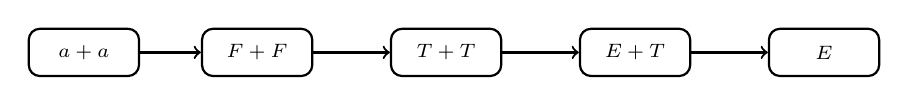
\begin{tikzpicture}[
    box/.style={
        draw,
        rounded corners,
        thick,
        minimum width=1.4cm,
        minimum height=0.6cm,
        align=center,
        font=\scriptsize
    },
    arrow/.style={->, thick}
]
    \node<5->[box] (s1) at (0,0) {$a + a$};
    \node<6->[box] (s2) at (2.2,0) {$F + F$};
    \node<7->[box] (s3) at (4.6,0) {$T + T$};
    \node<8->[box] (s4) at (7.0,0) {$E + T$};
    \node<9->[box] (s5) at (9.4,0) {$E$};

    \draw<6->[arrow] (s1) -- (s2);
    \draw<7->[arrow] (s2) -- (s3);
    \draw<8->[arrow] (s3) -- (s4);
    \draw<9->[arrow] (s4) -- (s5);
\end{tikzpicture}
